\section{Palíndromos}

%----------
% MT-0A
%----------

\subsection{MT Determinista de 1 cinta}

\subsubsection*{Diseño propuesto}
El algoritmo de resolución es el siguiente:

\begin{itemize}
    \item Ciclo:
    \begin{enumerate}[1.]
        \item Si no hay ninguna letra, poner un \texttt{1} (son palíndromos) y \textbf{parar}.
        \item Borrar una letra en el extremo izquierdo.
        \item Buscar la letra correspondiente en el extremo derecho.
        \item Si la letra coincide:
        \begin{enumerate}[1.]
            \item Borrarla.
            \item Volver al extremo izquierdo.
        \end{enumerate}
        \item En caso contrario:
        \begin{enumerate}[1.]
            \item Volver al extremo izquierdo, borrando todas las letras.
            \item Poner un \texttt{0} (no son palíndromos) y \textbf{parar}.
        \end{enumerate}
    \end{enumerate}
\end{itemize}

El diseño de la máquina queda representado en la Figura \ref{fig:MT-0A}.

\begin{figure}[h]
    \centering
    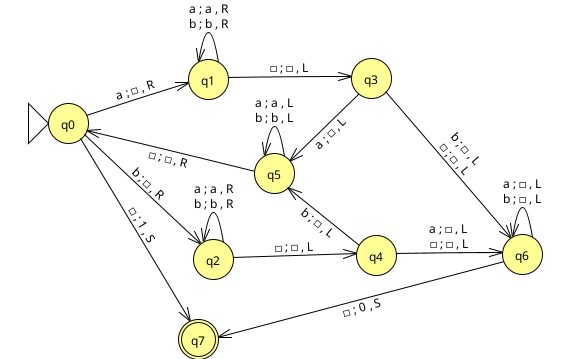
\includegraphics[width=0.7\textwidth]{MT-0A.png}
    \caption{Implementación en JFLAP de MT-0A}
    \label{fig:MT-0A}
\end{figure}


\subsubsection*{Peor caso}
El peor caso sería cuando es un palíndromo, dado que en el momento en el que una letra no coincida, deja de buscar el resto de letras. Dentro de los palíndromos, el peor caso es cuando es un palíndromo de tamaño par, ya que tiene que hacer una comprobación extra.

\subsubsection*{Evaluación empírica}
Realizamos la evaluación empírica en el peor caso, tomando como $n$ el tamaño de la palabra, y midiendo el número de pasos realizados para resolver el problema\footnote{Los datos se pueden encontrar en \texttt{data/MT-0A.csv}.}:

% TODO: use CSVsimple to generate table from csv files
\begin{table}[h]
    \centering
    \begin{tabular}{lcc}
        Entrada & $n$ & Pasos \\
        \hline
        $\lambda$               & 0  & 1  \\
        \texttt{aa}             & 2  & 6  \\
        \texttt{abba}           & 4  & 15 \\
        \texttt{abaaba}         & 6  & 28 \\
        \texttt{aaabbaaa}       & 8  & 45 \\
        \texttt{bbaabbaabb}     & 10 & 66 \\
        \texttt{bbbbbaabbbbb}   & 12 & 91
    \end{tabular}
\end{table}


\subsubsection*{Coste computacional}
Para obtener el coste computacional del algoritmo, aplicaremos Diferencias Finitas, basándonos en los datos de la evaluación empírica:

\begin{table}[H]
    \centering
    \begin{tabular}{|l|c|c|c|c|c|c|c|}
        \hline
        $n$ & \textbf{0} & \textbf{2} & \textbf{4} & \textbf{5} & \textbf{8} & \textbf{10} & \textbf{12} \\ \hline
        $T(n)$ & \textbf{1} & \textbf{6} & \textbf{15} & \textbf{28} & \textbf{45} & \textbf{66} & \textbf{91} \\ \hline
        \hline
        $A(n) = T(n) - T(n-2)$ &    &  5 &  9 & 13 & 17 & 21 & 25 \\ \hline
        $B(n) = A(n) - A(n-2)$ &    &    &  4 &  4 &  4 &  4 &  4 \\ \hline
        $C(n) = B(n) - B(n-2)$ &    &    &    &  0 &  0 &  0 &  0 \\ \hline
    \end{tabular}
    \label{tab:0A}
\end{table}

Al ser constantes las diferencias finitas segundas, y nulas las terceras, podemos aproximar $T(n)$ con un polinomio de segundo orden, es decir, $T(n) = an^2 + bn + c$.\\

Para obtener los valores de $a$, $b$, y $c$, usaremos valores de $n$ y $T(n)$ obtenidos en la evaluación empírica:

\begin{subequations}
    \begin{gather}
        n = 0,\ T(0) = 1 \rightarrow c = 1 \\
        n = 2,\ T(2) = 6 \rightarrow 4a + 2b + c = 6 \\
        n = 4,\ T(4) = 15 \rightarrow 16a + 4b + c = 6
    \end{gather}
\end{subequations}

Resolviendo, $a=\frac{1}{2}$ y $b=\frac{3}{2}$, por lo que:

\begin{equation}
    T_{\mathrm{0A}}(n) = 2n^2 + 6n + 2
\end{equation}


\subsubsection*{Cota asintótica}
La cota asintótica queda defida como:

\begin{equation}
    O(n) = k \cdot g(n) \geq T(n)
    \label{eq:On}
\end{equation}

Donde $g(n)$ representa el orden de la cota superior, en este caso $g(n) = n^2$.\\

Al conocer $T_{\mathrm{0A}}(n)$, si asumimos $n_0 = 10$, obtenemos $k \geq \frac{131}{50}$, por lo que la cota asintótica para esta máquina es:
\begin{equation}
    O_{\mathrm{0A}}(n) = \frac{131}{50} n^2
\end{equation}

Se puede observar la cota en comparación con el coste computacional en la Figura \ref{fig:MT-0A_plot} (asumiendo $n_0 = 10$).

\begin{figure}[h]
    \centering
    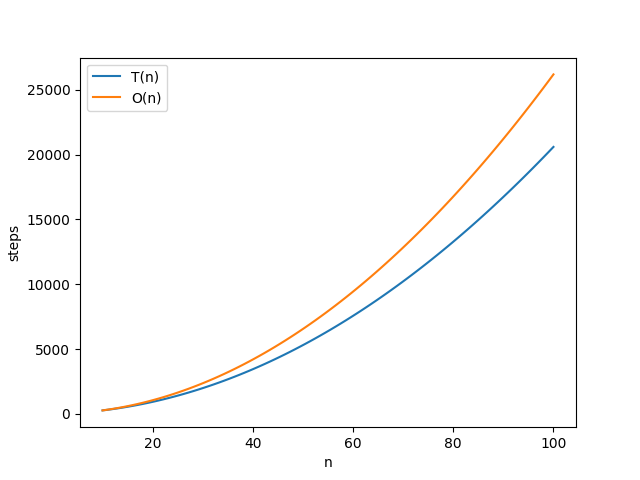
\includegraphics[width=0.6\textwidth]{plot_MT-0A_complexity.png}
    \caption{Coste computacional de MT-0A}
    \label{fig:MT-0A_plot}
\end{figure}


%----------
% MT-0B
%----------

\subsection{MT Determinista de 2 cintas}

\subsubsection*{Diseño propuesto}
El algoritmo de resolución es el siguiente:

\begin{enumerate}
    \item Copiar los símbolos de la cinta 0 a la cinta 1.
    \item Rebobinar la cinta 1.
    \item Cotejar los símbolos de la cinta 0 y la cinta 1, avanzando ambas cintas paso a paso, y borrando los símbolos.
    \begin{enumerate}[1.]
        \item Si en algún punto no coinciden, rebobinar la cinta 0, limpiar la cinta 1, poner un \texttt{0} (no son palíndromos) y \textbf{parar}.
    \end{enumerate}
    \item Poner un \texttt{1} (son palíndromos) y \textbf{parar}.
\end{enumerate}

El diseño de la máquina queda representado en la Figura \ref{fig:MT-0B}.

\begin{figure}[h]
    \centering
    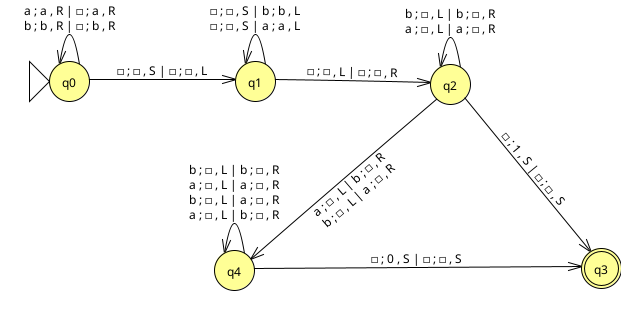
\includegraphics[width=0.8\textwidth]{MT-0B.png}
    \caption{Implementación en JFLAP de MT-0B}
    \label{fig:MT-0B}
\end{figure}

\subsubsection*{Peor caso}
El peor caso vuelve a ser un palíndromo par, puesto que tiene que comprobar toda la cadena.

\subsubsection*{Evaluación empírica}
Realizamos la evaluación empírica en el peor caso, tomando como $n$ el tamaño de la palabra, y midiendo el número de pasos realizados para resolver el problema\footnote{Los datos se pueden encontrar en \texttt{data/MT-0B.csv}.}:

\begin{table}[h]
    \centering
    \begin{tabular}{lcc}
        Entrada & $n$ & Pasos \\
        \hline
        $\lambda$               & 0  & 3  \\
        \texttt{aa}             & 2  & 9  \\
        \texttt{abba}           & 4  & 15 \\
        \texttt{abaaba}         & 6  & 21 \\
        \texttt{aaabbaaa}       & 8  & 27 \\
        \texttt{bbaabbaabb}     & 10 & 33 \\
        \texttt{bbbbbaabbbbb}   & 12 & 39
    \end{tabular}
\end{table}


\subsubsection*{Coste computacional}
Para obtener el coste computacional del algoritmo, aplicaremos Diferencias Finitas, basándonos en los datos de la evaluación empírica:

\begin{table}[H]
    \centering
    \begin{tabular}{|l|c|c|c|c|c|c|c|}
        \hline
        $n$ & \textbf{0} & \textbf{2} & \textbf{4} & \textbf{5} & \textbf{8} & \textbf{10} & \textbf{12} \\ \hline
        $T(n)$ & \textbf{3} & \textbf{9} & \textbf{15} & \textbf{21} & \textbf{27} & \textbf{33} & \textbf{39} \\ \hline
        \hline
        $A(n) = T(n) - T(n-2)$ &    &  6 &  6 &  6 &  6 &  6 &  6 \\ \hline
        $B(n) = A(n) - A(n-2)$ &    &    & 0 &  0 &  0 &  0 &  0 \\ \hline
    \end{tabular}
    \label{tab:0B}
\end{table}

Al ser constantes las diferencias finitas primeras, y nulas las segundas, podemos aproximar $T(n)$ con un polinomio de primer orden, es decir, $T(n) = an + b$.\\

Para obtener los valores de $a$ y $b$, usaremos valores de $n$ y $T(n)$ obtenidos en la evaluación empírica:

\begin{subequations}
    \begin{gather}
        n = 0,\ T(0) = 3 \rightarrow b = 3 \\
        n = 2,\ T(2) = 9 \rightarrow 2a + b = 9
    \end{gather}
\end{subequations}

Resolviendo, $a=b=3$, por lo que:

\begin{equation}
    T_{\mathrm{0B}}(n) = 3n + 3
    \label{eq:Tn0B}
\end{equation}

También podemos calcular el coste computacional mediante una evaluación analítica del algoritmo. MT-0B realiza tres recorridos, en el peor de los casos:
\begin{enumerate}
    \item Copia los datos de la cinta 0 a la cinta 1 $\rightarrow n+1$ pasos
    \item Rebobina la cinta 1 $\rightarrow n+1$ pasos
    \item Coteja la cinta 1 con la cinta 2, en reverso $\rightarrow n+1$ pasos
\end{enumerate}

Sumando los tres recorridos, nos queda el mismo resultado que en la ecuación \ref{eq:Tn0B}.


\subsubsection*{Cota asintótica}
Al conocer $T_{\mathrm{0B}}(n)$, podemos afirmar que $g(n) = n$. Si asumimos $n_0 = 10$, obtenemos $k \geq \frac{33}{10}$, por lo que la cota asintótica (definida en la ecuación \ref{eq:On}) para esta máquina es:
\begin{equation}
    O_{\mathrm{0B}}(n) = \frac{33}{10} n
\end{equation}


Se puede observar la cota en comparación con el coste computacional en la Figura \ref{fig:MT-0B_plot} (asumiendo $n_0 = 10$).

\begin{figure}[h]
    \centering
    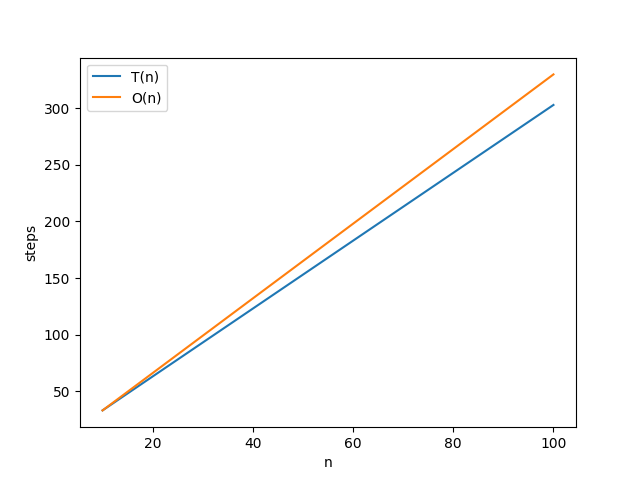
\includegraphics[width=0.6\textwidth]{plot_MT-0B_complexity.png}
    \caption{Coste computacional de MT-0B}
    \label{fig:MT-0B_plot}
\end{figure}


%----------
% MT-0C
%----------

\subsection{MT No Determinista de 2 cintas}

\subsubsection*{Diseño propuesto}
El algoritmo de resolución es el siguiente:

\begin{enumerate}
    \item Copiar la primera mitad de la palabra a la segunda cinta. Al ser no determinista, asumimos a cada paso que hemos llegado a la mitad y pasamos al siguiente paso.
    \item Cotejar ambas cintas, leyendo la cinta 1 en reverso y avanzando la cinta 0, y borrando ambas cintas a su paso. En el momento en el que no coincidan los elementos de ambas cintas, acaba sin llegar a un estado final, por lo que la palabra no es aceptada.
    \item Poner un 1 en la cinta 0 y \textbf{parar}.
\end{enumerate}

El diseño de la máquina queda representado en la Figura \ref{fig:MT-0C}.

\begin{figure}[h]
    \centering
    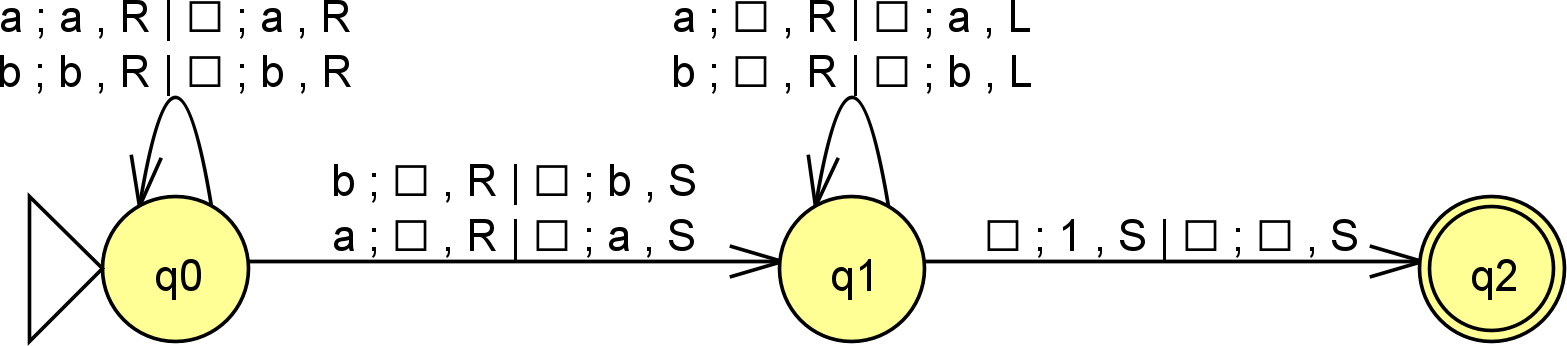
\includegraphics[width=0.6\textwidth]{MT-0C.png}
    \caption{Implementación en JFLAP de MT-0C}
    \label{fig:MT-0C}
\end{figure}

\subsubsection*{Peor caso}
El peor caso vuelve a ser un palíndromo par, puesto que tiene que comprobar toda la cadena, y en caso de que no sea un palíndromo acaba antes.


\subsubsection*{Evaluación empírica}
Realizamos la evaluación empírica en el peor caso, tomando como $n$ el tamaño de la palabra, y midiendo el número de pasos realizados para resolver el problema\footnote{Los datos se pueden encontrar en \texttt{data/MT-0C.csv}.}:

\begin{table}[h]
    \centering
    \begin{tabular}{lcc}
        Entrada & $n$ & Pasos \\
        \hline
        \texttt{aa}             & 2  & 4 \\
        \texttt{abba}           & 4  & 6 \\
        \texttt{abaaba}         & 6  & 8 \\
        \texttt{aaabbaaa}       & 8  & 10 \\
    \end{tabular}
\end{table}

\subsubsection*{Coste computacional}
Para obtener el coste computacional del algoritmo, aplicaremos Diferencias Finitas, basándonos en los datos de la evaluación empírica:

\begin{table}[H]
    \centering
    \begin{tabular}{|l|c|c|c|c|}
        \hline
        $n$ & \textbf{2} & \textbf{4} & \textbf{6} & \textbf{8} \\ \hline
        $T(n)$ & \textbf{4} & \textbf{6} & \textbf{8} & \textbf{10} \\ \hline
        \hline
        $A(n) = T(n) - T(n-2)$ &   & 2 & 2 & 2 \\ \hline
        $B(n) = A(n) - A(n-2)$ &   &   & 0 & 0 \\ \hline
    \end{tabular}
    \label{tab:0C}
\end{table}

Al ser constantes las diferencias finitas primeras, y nulas las segundas, podemos aproximar $T(n)$ con un polinomio de primer orden, es decir, $T(n) = an + b$.\\

Para obtener los valores de $a$ y $b$, usaremos valores de $n$ y $T(n)$ obtenidos en la evaluación empírica:

\begin{subequations}
    \begin{gather}
        n = 2,\ T(2) = 4 \rightarrow 2a + b = 4 \\
        n = 4,\ T(4) = 6 \rightarrow 4a + b = 6
    \end{gather}
\end{subequations}

Resolviendo, $a = 1$ y $b=2$, por lo que:

\begin{equation}
    T_{\mathrm{0C}}(n) = n + 2
\end{equation}


\subsubsection*{Cota asintótica}
Al conocer $T_{\mathrm{0B}}(n)$, podemos afirmar que $g(n) = n$. Si asumimos $n_0 = 10$, obtenemos $k \geq \frac{12}{10}$, por lo que la cota asintótica (definida en la ecuación \ref{eq:On}) para esta máquina es:
\begin{equation}
    O_{\mathrm{0C}}(n) = \frac{12}{10} n
\end{equation}

Se puede observar la cota en comparación con el coste computacional en la Figura \ref{fig:MT-0C_plot} (asumiendo $n_0 = 10$).

\begin{figure}[h]
    \centering
    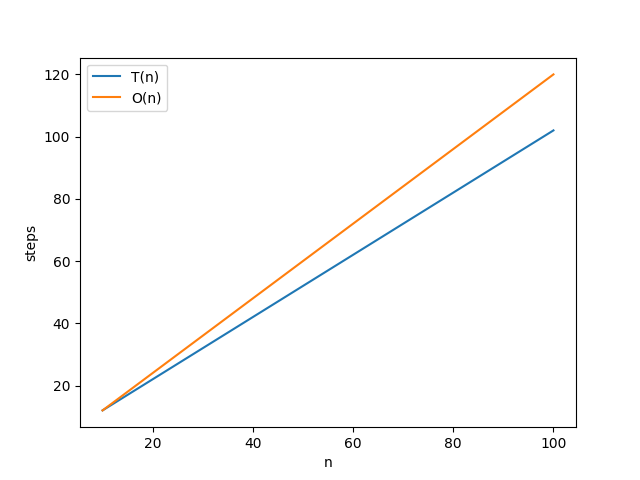
\includegraphics[width=0.6\textwidth]{plot_MT-0C_complexity.png}
    \caption{Coste computacional de MT-0C}
    \label{fig:MT-0C_plot}
\end{figure}